\section{Modeling of Fake Backgrounds}
\label{sec:introduction}
Fake backgrounds for \Bmumu arise mainly from the misidentification of final-state hadrons (mostly pions and kaons) as muons. %
In particular, the decays of the form $B_{(s)}\to hh'$ (where $h,h'$ are hadrons) are expected to form a peaking background when both the hadrons in the final state are misidentified as muons. %
Since all decays with one muon in the final state necessarily also have a neutrino in the final state, $B_{(s)}\to hh'$ decays are the only source of peaking background in this analysis. %
Due to the extremely low branching ratio (\(\sim \mathcal{O}(10^{-10})\)) of the \Bmumu decays, their measurement is expected to be quite sensitive to the estimation of such fake background despite the anticipated $\mathcal{O}(10^{-3})$ probability for a hadron to be misidenitifed as a muon. %
\\\\
The difficulty in modeling fake backgrounds with MC simulation arises from the difficulty to accurately model the interaction of hadrons with the calorimeters (including the details of shower development) in MC simulation.
The mechanism by which hadrons leave signatures in the detector that resemble those of leptons primarily depends on their behavior in the calorimeter. In the case of faking muons, it depends on whether they can escape the hadronic calorimeter and leave a signature in the muon spectrometer. Because MC simulations have limitations in accurately modeling these hadron–calorimeter interactions, the analysis of fake backgrounds needs to be at least partially data-driven. 
While peaking and combinatorial backgrounds can be modeled to some extent with MC simulation, fake backgrounds remain difficult to model accurately due to the complexity of hadron–calorimeter interactions and the low probability of hadrons faking muons (\(\sim \mathcal{O}(10^{-3})\)), which makes MC simulation computationally expensive to obtain a good estimate of the fake backgrounds in MC simulation.

\subsection{Outline of the Strategy}
\label{subsec:outline-of-strategy}

The data-driven method for estimating fake backgrounds in the \Bmumu analysis consists of two main steps:

\begin{itemize}
    \item \textbf{Estimation of the Faking Probabilities}: Calculate, from data (for kaons) or MC (for pions), the probability that a hadron fakes a muon.
    \item \textbf{Estimation of the Fake Background}: Use these probabilities to estimate the background in the signal region of the analysis.
\end{itemize}

\subsubsection{Estimation of the Faking Probabilities}
\label{subsubsec:estimation-of-faking-probabilities}

To estimate the probability that a hadron \( h \) fakes a muon, we use a control region where hadrons are the dominant source of reconstructed muons. %
%In "traditional" analyses, the control region is often obtained by inverting the leptons' identification criteria. However, such an approach is not directly amenable to \( B \)-physics analysis.
%\begin{itemize}
%    \item The “traditional” analyses typically target isolated, prompt leptons. Here, ``prompt'' means that they do not originate from decays-in-flight, i.e., from heavy-flavor decays; ``isolated'' means that there is not much hadronic activity around the lepton in the calorimeter and/or in the tracker. The variables used to discriminate between a region dominated by real leptons and fake leptons rely on the assumption of high$-p_{\text{T}}$ prompt leptons, e.g., inverting the cut on the lepton identification measure or inverting the isolation variables. %
%    However, since the signal leptons in $B$-physics analyses come from $B$-decays, they are not very isolated as they lie in the vicinity of the decay products of the primary vertex in which the $B$-meson originated. %
%    \item Even if a variable can be found whose selection can be inverted to differentiate between signal leptons and fake leptons, extracting a fake-enrinched region via subtracting the non-fake backgrounds is much less straightforward compared to the “traditional” analyses where the real background component is usually defined by a small set of well modeled processes (typically top and electroweak processes). %
%    In particular, the fake-lepton contributions in this control region, just like the signal in the signal region, will be swamped by combinatorial as well as partially reconstructed decays. 
%\end{itemize}
%We thus need to develop a different approach to obtain a fake-enriched region. %
We follow the approach outlined in \textbf{CITE FABIOLA'S QT REPORT and RUN1 paper} wherein we utilize the decays of $B$-hadrons to unambiguously identify hadrons and thus isolate a hadron-enriched region that we then use to derive the faking probabilities of the said hadron. %
To estimate the probability that a hadron $h$ fakes a muon, i.e., $P(h\rightarrow\mu)$, we first identify a decay channel of a heavier hadron that can be used to tag the hadron of interest. %
A natural choice for the parent hadron is a $B$-hadron since it automatically puts us in a phase-space that is not dissimilar to the phase-space that would be occupied by hadrons faking leptons in our analysis. %
Specifically, we use the decay channel $B^+\to J/\psi(\to \mu^+\mu^-)K^+$ to tag kaons and estimate the probability \( P(K^\pm \rightarrow \mu^\pm) \). The same approach is used for pions via the decay channel $B^+\to J/\psi(\to \mu^+\mu^-)\pi^+$. However, since we cannot distinguish between kaons and pions, combined with the fact that this decay is CKM suppressed, it cannot be effectively isolated in data. We thus estimate the probability \( P(K^\pm \rightarrow \mu^\pm) \) from the MC samples of the $B^+\to J/\psi(\to \mu^+\mu^-)\pi^+$ decay. Notice that kaons have a significantly higher probability to fake a muon than pions, thus, the potential inaccuracy in the MC-based estimation of \( P(K^\pm \rightarrow \mu^\pm) \) is expected to be negligible\footnote{We can, in principle, utilize the decay \( B^0 \rightarrow J/\psi(\mu^+\mu^-)K^{*0}(\rightarrow K^+\pi^-) \), allowing us to estimate \( P(\pi^\pm \rightarrow \mu^\pm) \) from data. While ATLAS cannot effectively discriminate between the $K^\pm$ and $\pi^\pm$, the fact that they come from a common $K^{\ast 0}$-vertex provides us with a good enough handle on their particle identification -- based on checking if assigning the $K^+$ mass hypothesis to the positively charged meson (and $\pi^-$ mass hypothesis to the negatively charged meson) leads to a dimeson mass that is closer to the PDG value of the $K^{\ast 0}$ mass compared to reverting the mass-hypothesis assignments.}.

The faking probability is calculated as:
\[
P(h \rightarrow \mu^\pm) = \frac{N_{h \rightarrow \mu^\pm}}{N_h}
\]
where \( N_{h \rightarrow \mu^\pm} \) is the number of hadrons that are reconstructed as muons, and \( N_h \) is the total number of tagged hadrons.

We derive the following faking probabilities using this approach: 
\begin{itemize}
    \item $P(K^\pm \to \mu^\pm)$
    \item $P(\pi^\pm \to \mu^\pm)$
\end{itemize}

where, in this context, $\rightarrow\equiv \xrightarrow[\text{reconstructed as}]{}$ and \underline{not} a decay (albeit some of the misidentifications come from in-flight decays). 
\subsubsection{Estimation of the Fake Background}
\label{subsubsec:estimation-of-fake-background}

Once the faking probabilities are known, the fake background in the signal region is estimated by applying these probabilities to MC samples of background processes that can contribute to a peaking fake background. However, it is important to note that we do not rely on the MC modeling of the process through which a hadron fakes a lepton, rather, we will utilize the faking probabilities that we derived in the previous section by selecting the relevant hadrons in the MC sample and assigning them with the relevant probability to fake a lepton. What we are utilizing from the MC simulation is the decay kinematics. The strategy is as follows:

\begin{itemize}
    \item \textbf{Prepare MC Samples}: Generate MC samples for all decays that can reasonably contribute to a fake background peaking in the signal region. For \Bmumu, these are mainly \( B_{(s)}^0 \rightarrow K^\pm K^\mp \), \( B_{(s)}^0 \rightarrow \pi^\pm K^\mp \), \( B_{(s)}^0 \rightarrow K^\pm \pi^\mp \), and \( B_{(s)}^0 \rightarrow \pi^\pm \pi^\mp \).
    \item \textbf{Perform Analysis Without Lepton Identification Cuts}: Run the analysis on these MC samples without requiring muon identification cuts.
    \item \textbf{Apply Faking Probabilities}: Weight each event by the faking probability derived from data.
    \item \textbf{Kinematic Corrections}: Correct for differences in track reconstruction between hadron and muon tracks.
    \item \textbf{Trigger Weights}: Correct for the removal of online (trigger-level) muon identification cuts using weights derived from a reference channel.
\end{itemize}
\subsection{Detailed Methodology}
\label{subsec:detailed-methodology}

\subsubsection{Estimation of $P(K^\pm\to\mu^\pm)$}
\label{subsubsec:estimation-of-K-to-ell}
The faking probabilities of the kaons are derived using the decay channel $B^\pm\to J/\psi(\to \mu^+\mu^-)K^\pm$. %
In particular, the $B^\pm\to J/\psi(\to \mu^+\mu^-)K^\pm$ candidates are reconstructed by fitting two well-identified muon tracks and an additional charged track to a common vertex. %
No particle identification criteria are applied to the additional charged track. %
Simple cuts on the quality of the $B$-vertex fit, the displacement of the $B$-vertex from the primary vertex, and the pointing angle are applied to suppress the combinatorial background. %
Finally, the reconstructed mass of the $B^\pm$-meson is calculated after constraining the mass of the dimuon system to the PDG value of the $J/\psi$ mass. %
Now, two yields are extracted:
\begin{itemize}
    \item The yield of all of the $B^\pm$-candidates is obtained using an unbinned extended maximum likelihood fit to the reconstructed mass of the $B^\pm$-candidates. %
    This yield is our roundabout way of obtaining the number of kaons, i.e., $N_{K^\pm}$. Recall that we are not really interested in the $B^\pm$-decay itself, but rather, we simply use this decay to tag the kaons. An example mass fit to the reconstructed $B$-mass to extract the yield of $N_{K^\pm}$ is shown in \ref{fig:fakeMuonMassFitForKaons} (left). %
    \item We select a subset of the $B^+$-candidates wherein we can match the ID track of the kaon to the ID track of a reconstructed lepton (at a given lepton identification working point). The yield of all such $B^+$-candidates is now obtained using an unbinned extended maximum likelihood fit to the reconstructed mass of the $B^+$-candidates. %
    This yield is our roundabout way of obtaining the number of kaons that fake a lepton, i.e., $N_{K^\pm\rightarrow\mu^\pm}$. %
    An example mass fit to the reconstructed $B$-mass to extract the yield of $N_{K^\pm\to\mu^\pm}$ is shown in \ref{fig:fakeMuonMassFitForKaons} (right). %
\end{itemize}
\begin{figure}[!ht]
    \centering 
    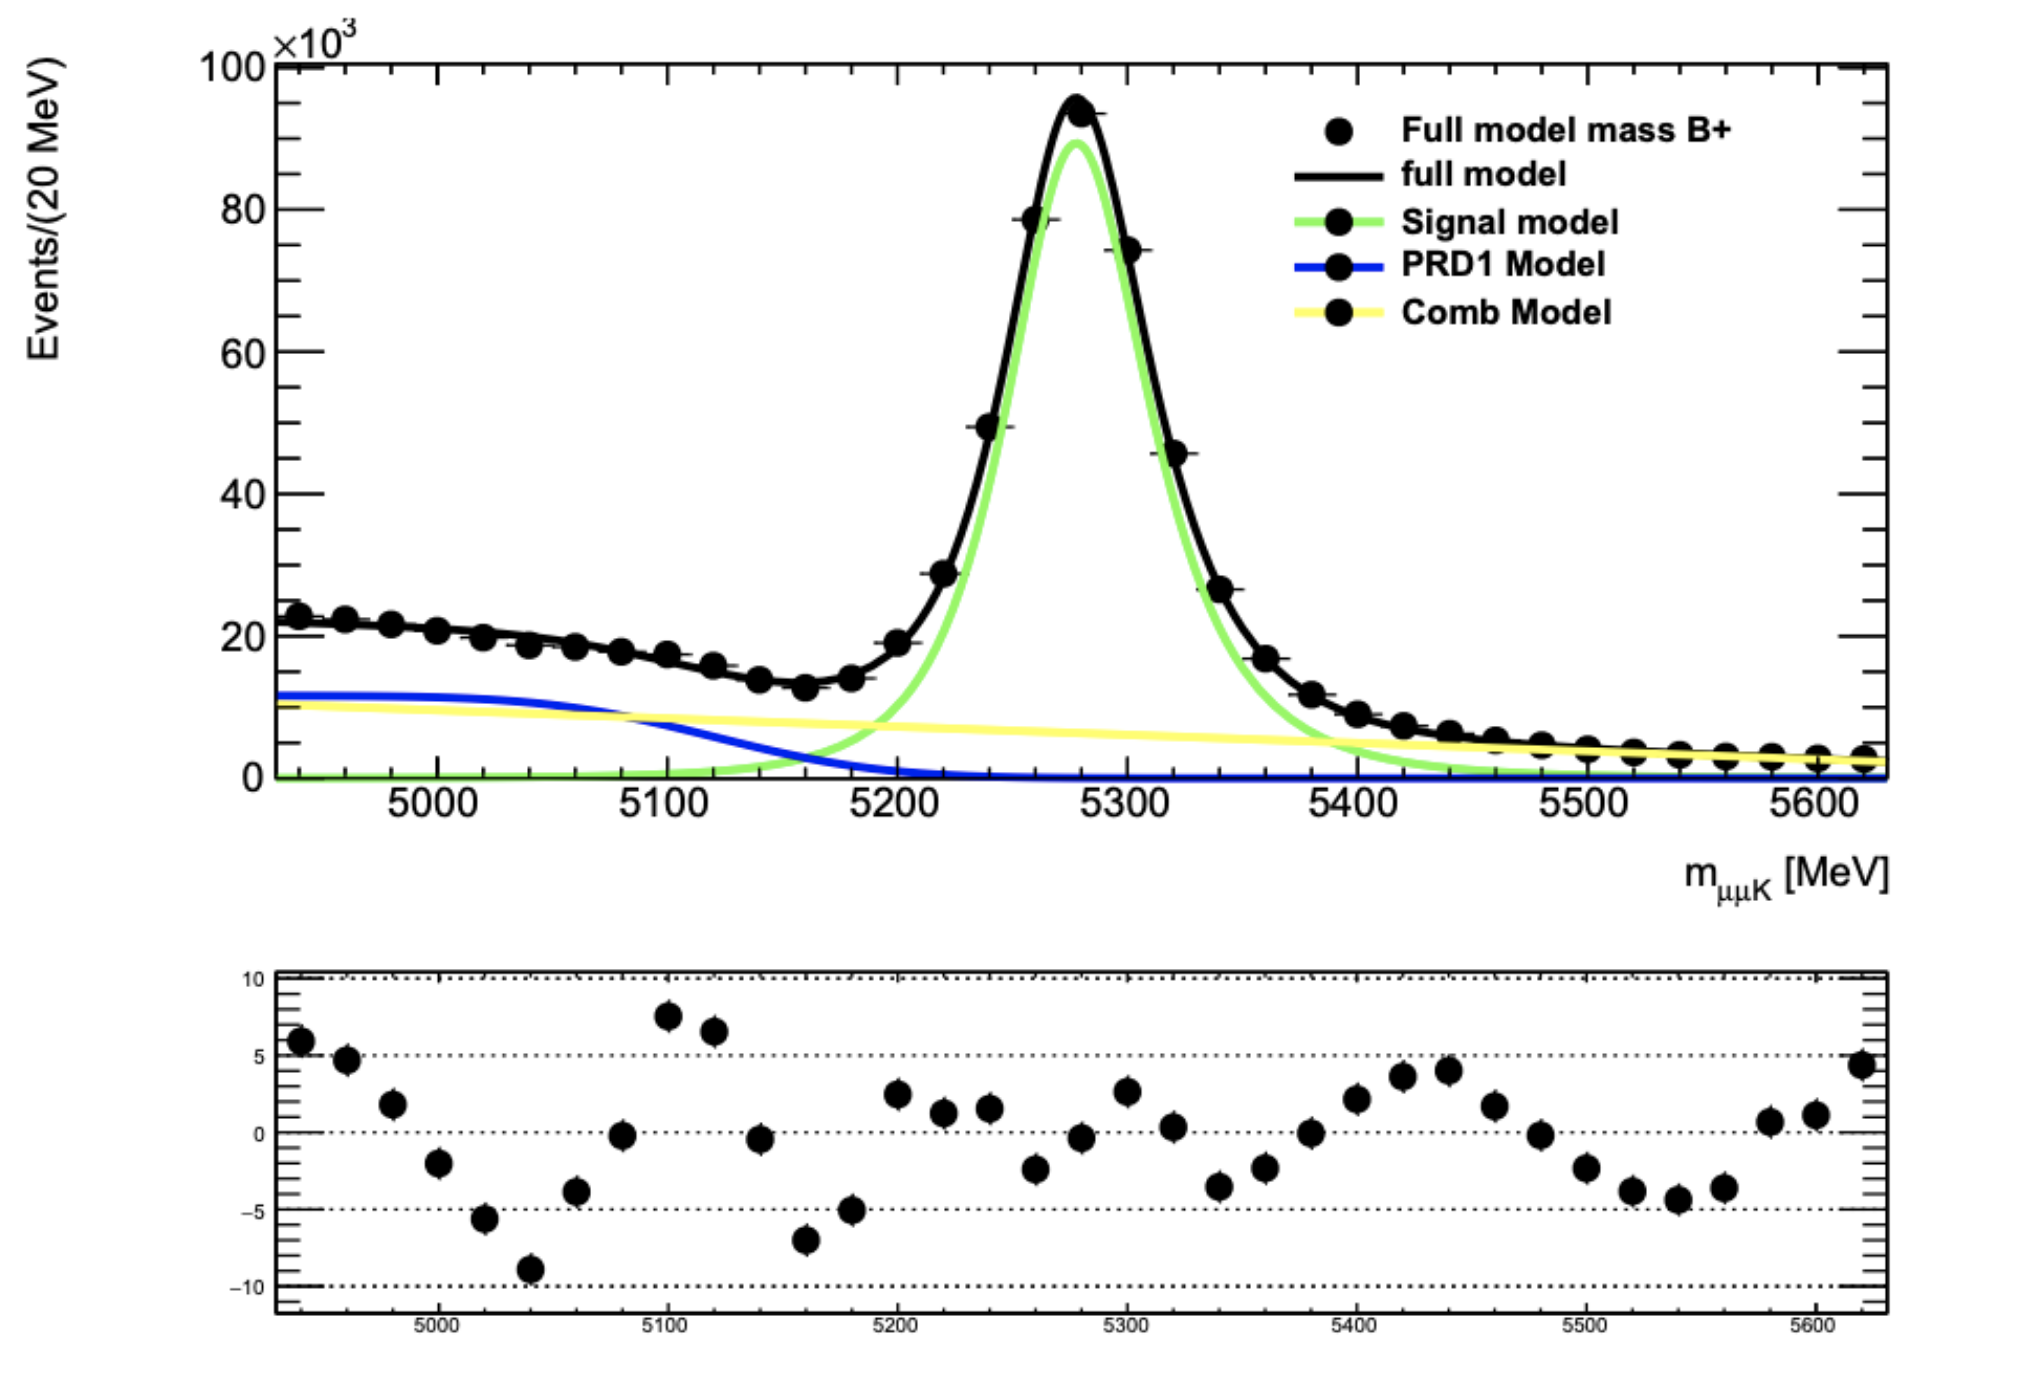
\includegraphics[width=0.45\textwidth]{figures/FakeRatesFit/fakeMuonFitDenom.png}
    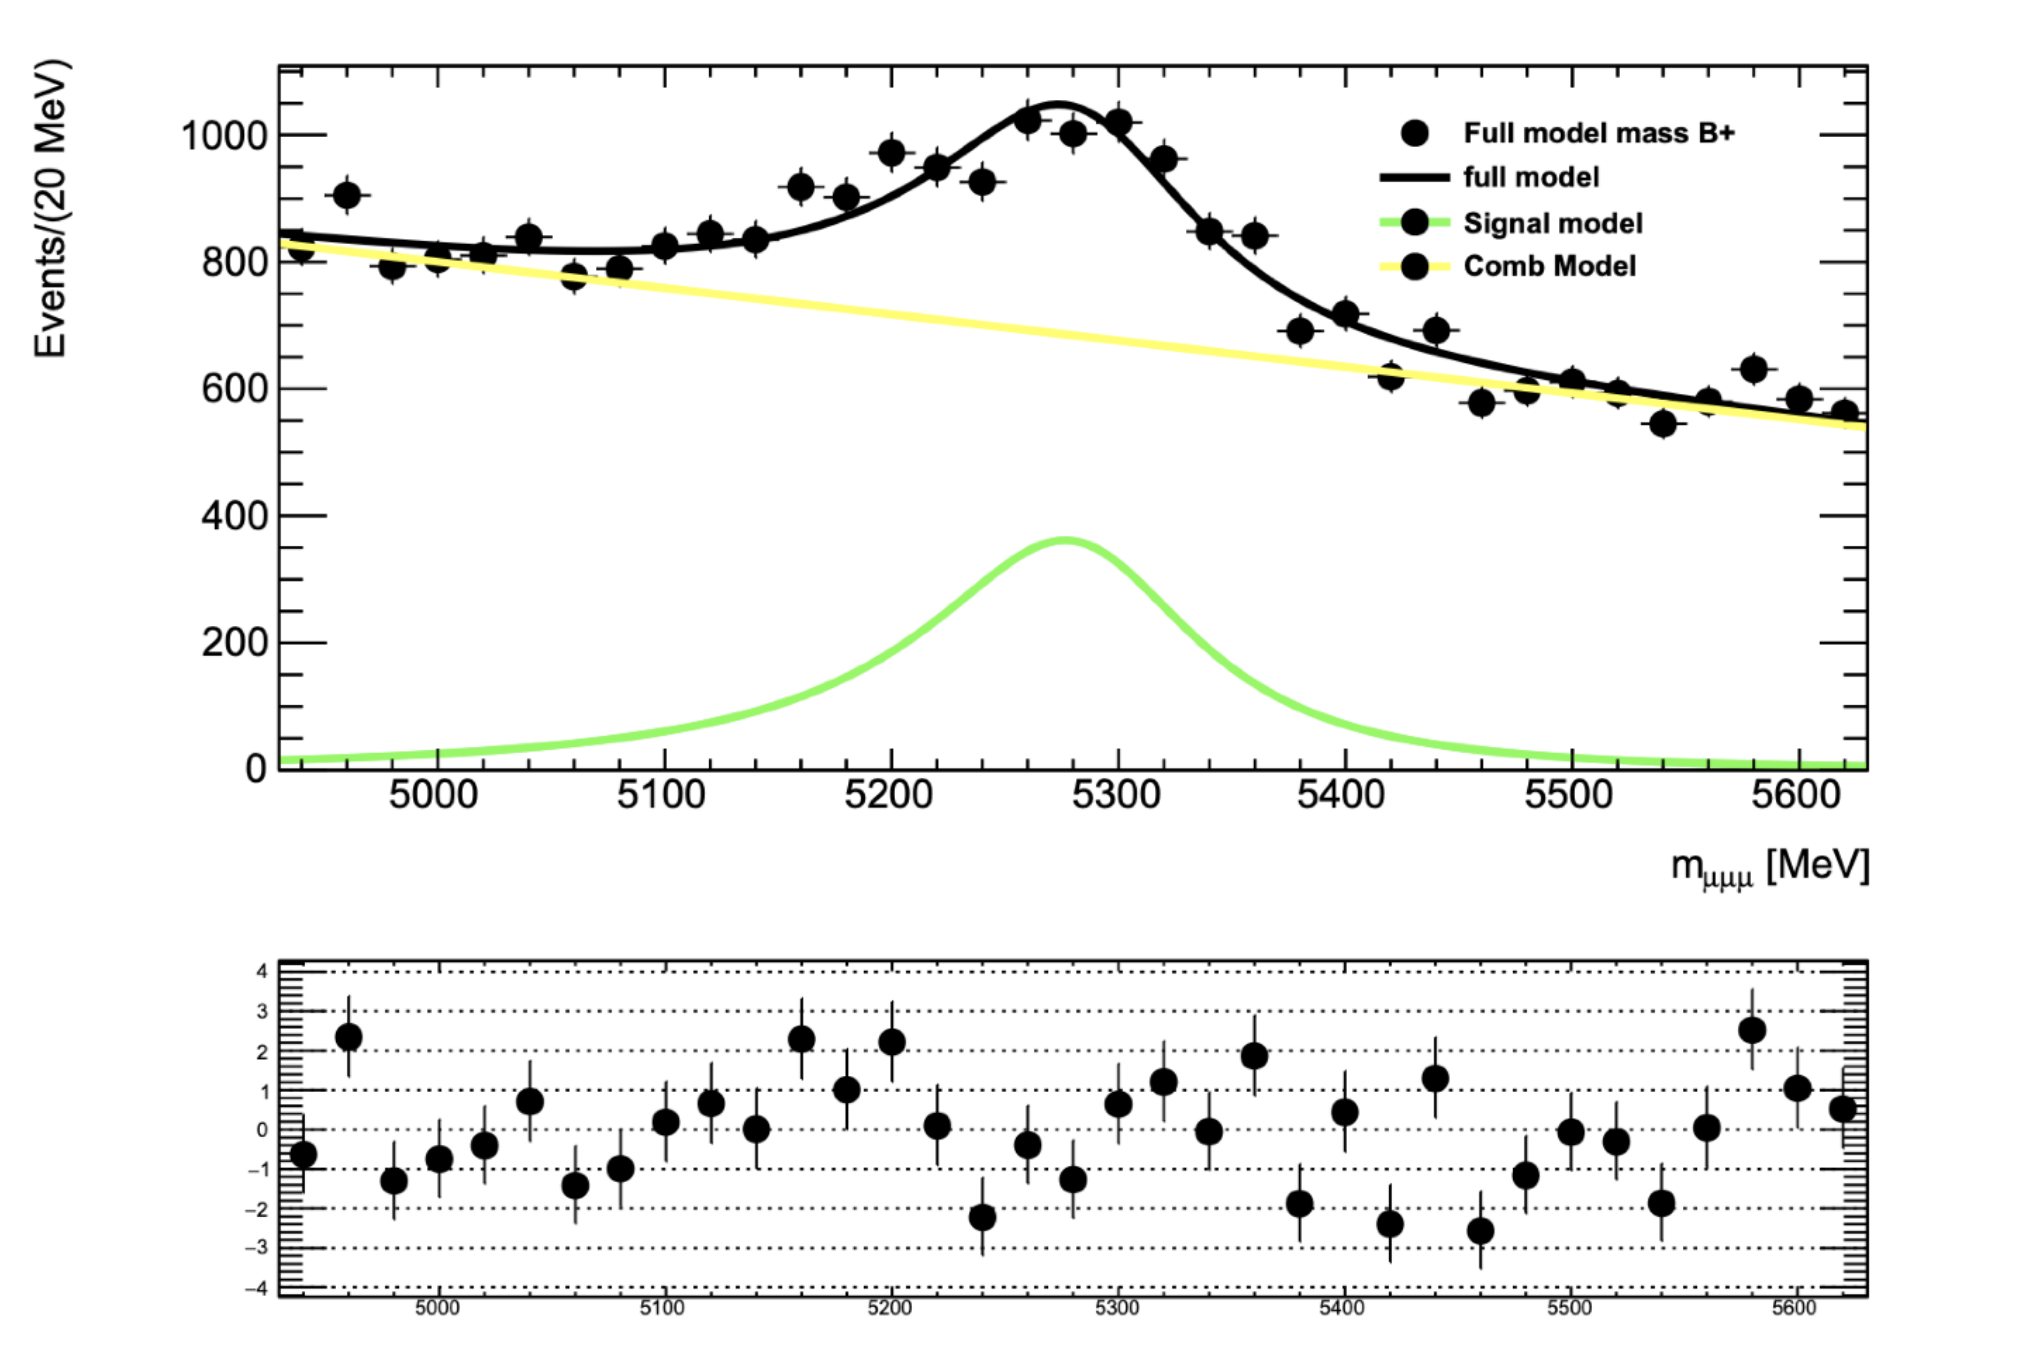
\includegraphics[width=0.45\textwidth]{figures/FakeRatesFit/fakeMuonFitNumer.png}
    \caption{Example mass fit to the reconstructed $B$-mass to extract the yield of $N_{K^\pm}$ (left) and $N_{K^\pm\to\mu^\pm}$ (right).}
    \label{fig:fakeMuonMassFitForKaons}
\end{figure}
Finally, the faking probability of the kaons is obtained as:
\begin{equation}
    P(K^\pm\to\mu^\pm) = \frac{N_{K^\pm\to\mu^\pm}}{N_{K^\pm}}
\end{equation}
This procedure is repeated in bins of $p_{\text{T}}$ of the kaon ID track for both the Barrel and the Endcap regions of the ATLAS detector. %
The results for the faking probabilities of the kaons are shown in \ref{fig:K-to-ell-faking-probabilities} (left). The fit results for all bins in the $p_{\text{T}} - \eta$ space are given in the Appendices ~\ref{subsec:Fake_Rates_Fits_Kaon} - ~\ref{subsec:Fake_Rates_Fits_Kaon_Muon}%

\subsubsection{Estimation of $P(\pi^\pm \to \mu^\pm)$}
The faking probabilities of the pions are derived using the decay channel $B^0\to J/\psi(\to \mu^+\mu^-)K^{\ast 0}(\to K^+\pi^-)$. %
The $B^0$-candidates are reconstructed by fitting two well-identified muon tracks and two additional charged tracks to a common vertex. %
No particle identification criteria are applied to the additional charged tracks (recall that ATLAS cannot effectively distinguish between different mesons, certainly not above $1{\ {\text{ GeV}}}$). %
Simple cuts on the quality of the $B$-vertex fit, the displacement of the $B$-vertex from the primary vertex, and the pointing angle are applied to suppress the combinatorial background. %
At this point, we check if assigning the $K^+$ mass hypothesis to the positively charged meson (and $\pi^-$ mass hypothesis to the negatively charged meson) leads to a dimeson mass that is closer to the PDG value of the $K^{\ast 0}$ mass compared to reverting the mass-hypothesis assignments. %
Depending on which mass hypothesis assignment leads to a dimeson mass that is closer to the PDG value of the $K^{\ast 0}$ mass, we assign the positively charged meson as either a $K^+$ or a $\pi^+$ and the negatively charged meson as either a $\pi^-$ or a $K^-$. %

This assignment is then used for two different purposes:
\begin{itemize}
    \item The assigned mass hypotheses are used to calculate the reconstructed $B^0$-meson mass. %
    \item The assigned mass hypotheses are also used to isolate the $\pi^\pm$ from the $K^\mp$ in the calculation of the faking probabilities. For example, in the following, we will focus on deriving the faking probabilities of the positively charged meson, i.e., $P(\pi^+ \to \mu^+)$. The negatively charged meson is treated in a similar way. %
\end{itemize}
In order to isolate the subset of $B^0$-candidates wherein the positively charged meson track is a $\pi^+$, we simply select the subset wherein the positively charged meson track is assigned the $\pi^+$ mass hypothesis via the procedure described above. %
Finally, the reconstructed mass of the $B^{\ast 0}$-meson is calculated after constraining the mass of the dimuon system to the PDG value of the $J/\psi$ mass. %
Now, two yields are extracted:
\begin{itemize}
    \item The yield of all of the $B^0$-candidates is obtained using an unbinned extended maximum likelihood fit to the reconstructed mass of the $B^0$-candidates. %
    This yield is our roundabout way of obtaining the number of positively charged pions, i.e., $N_{\pi^+}$. Recall that we are not really interested in the $B^0$-decay itself, but rather, we simply use this decay to tag the pions.
    \item We select a subset of the $B^0$-candidates wherein we can match the ID track of the (positively charged) pion to the ID track of a (positively charged) reconstructed lepton (at a given lepton identification working point). The yield of all such $B^0$-candidates is now obtained using an unbinned extended maximum likelihood fit to the reconstructed mass of the $B^0$-candidates. %
    This yield is our roundabout way of obtaining the number of (positively charged) pions that fake a (positively charged) lepton, i.e., $N_{\pi^+\to\mu^+}$. %
\end{itemize}
Finally, after repeating the equivalent procedure for the negatively charged pions, the faking probability of the pions is obtained as:
\begin{equation}
    P(\pi^\pm\to\mu^\pm) = \frac{N_{\pi^\pm\to\mu^\pm}}{N_{\pi^\pm}}
\end{equation}
This procedure is repeated in bins of $p_{\text{T}}$ of the pion ID track for both the Barrel and the Endcap regions of the ATLAS detector. %
The results for the faking probabilities of the pions are shown in \ref{fig:K-to-ell-faking-probabilities} (right). %
It should be noted that the faking probabilities that are shown here are from MC, and the equivalent probabilities are not yet derived using data (as the relevant data samples needed for performing this analysis are yet in the production stage). The fit results for all bins in the $p_{\text{T}} - \eta$ space are given in the Appendices ~\ref{subsec:Fake_Rates_Fits_Pion} - ~\ref{subsec:Fake_Rates_Fits_Pion_Muon}%
\begin{figure}[!ht]
    \centering 
    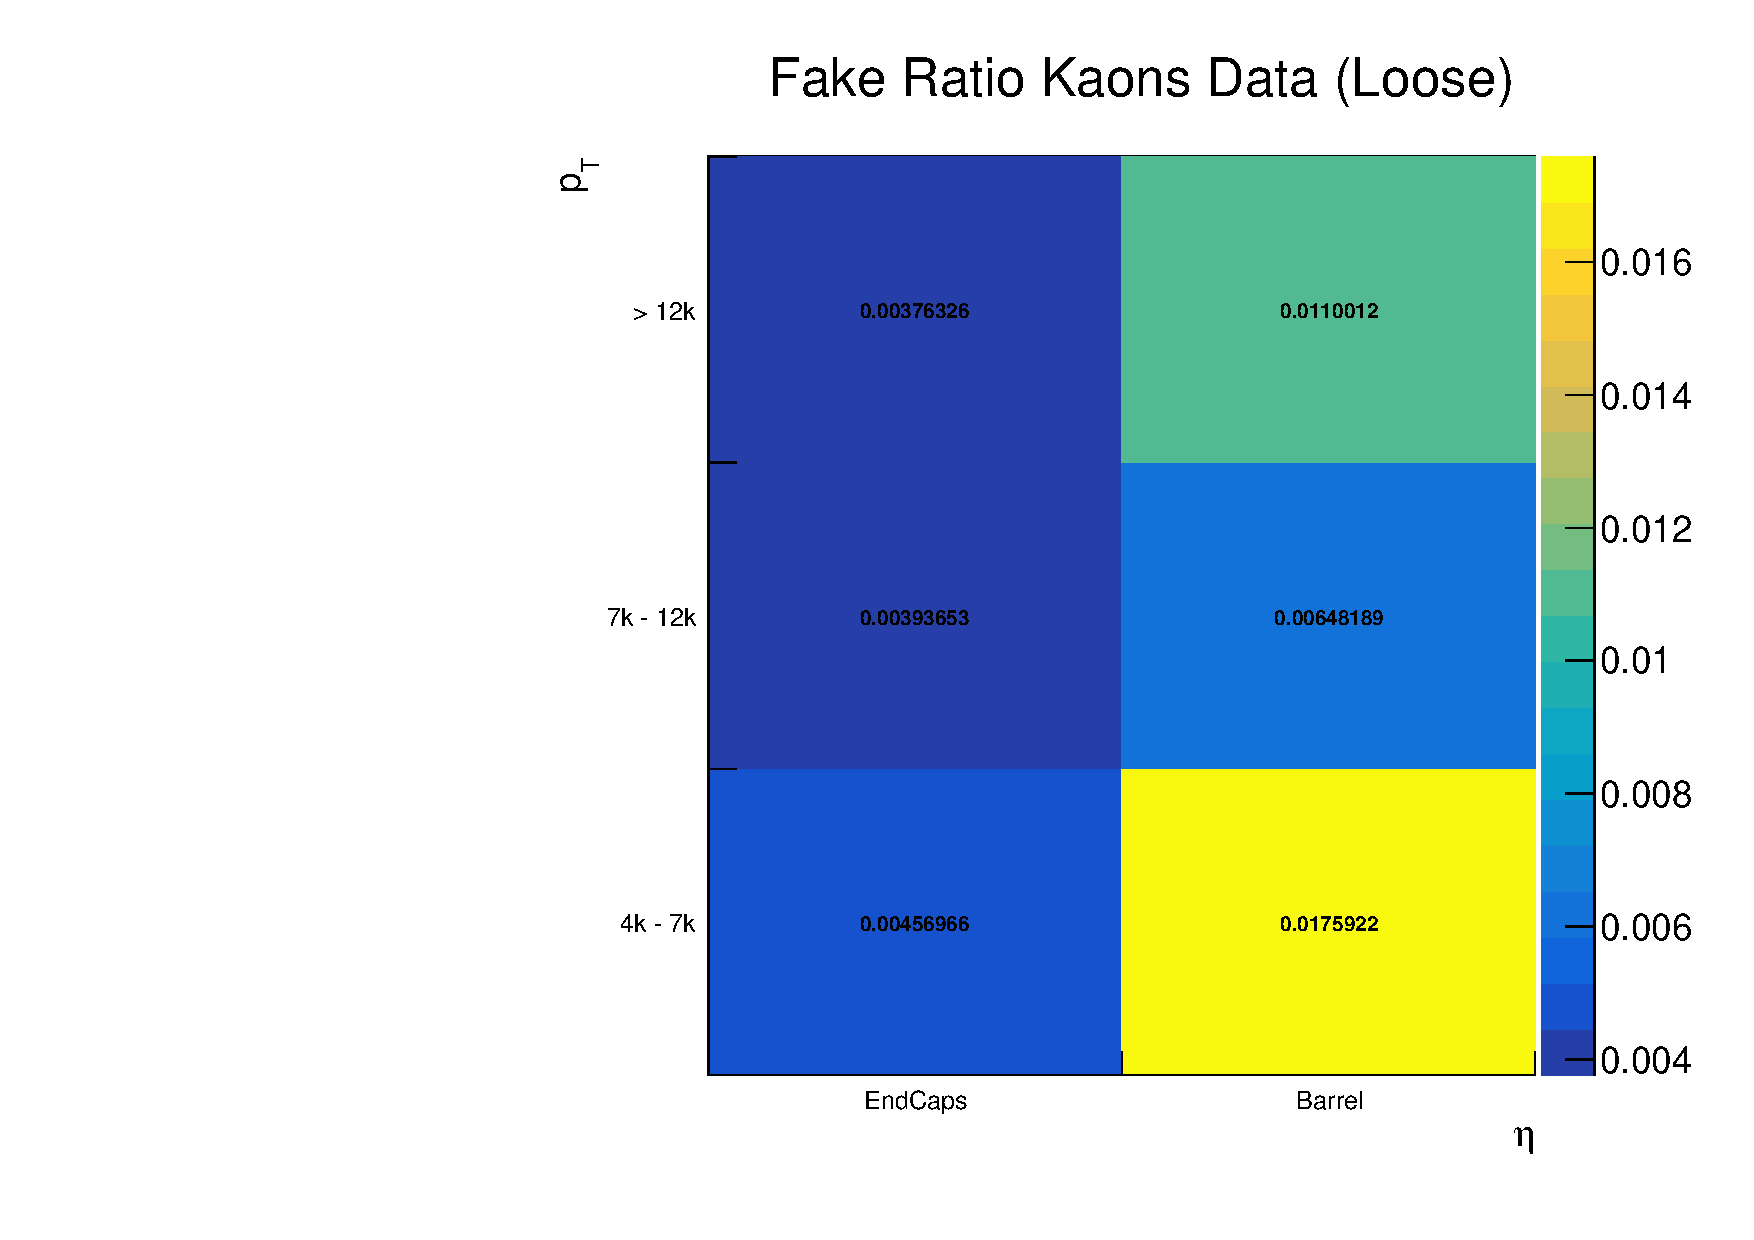
\includegraphics[width=0.45\textwidth]{figures/FakeRatesFit/FakeRates/FakeRatesLoose.pdf}
    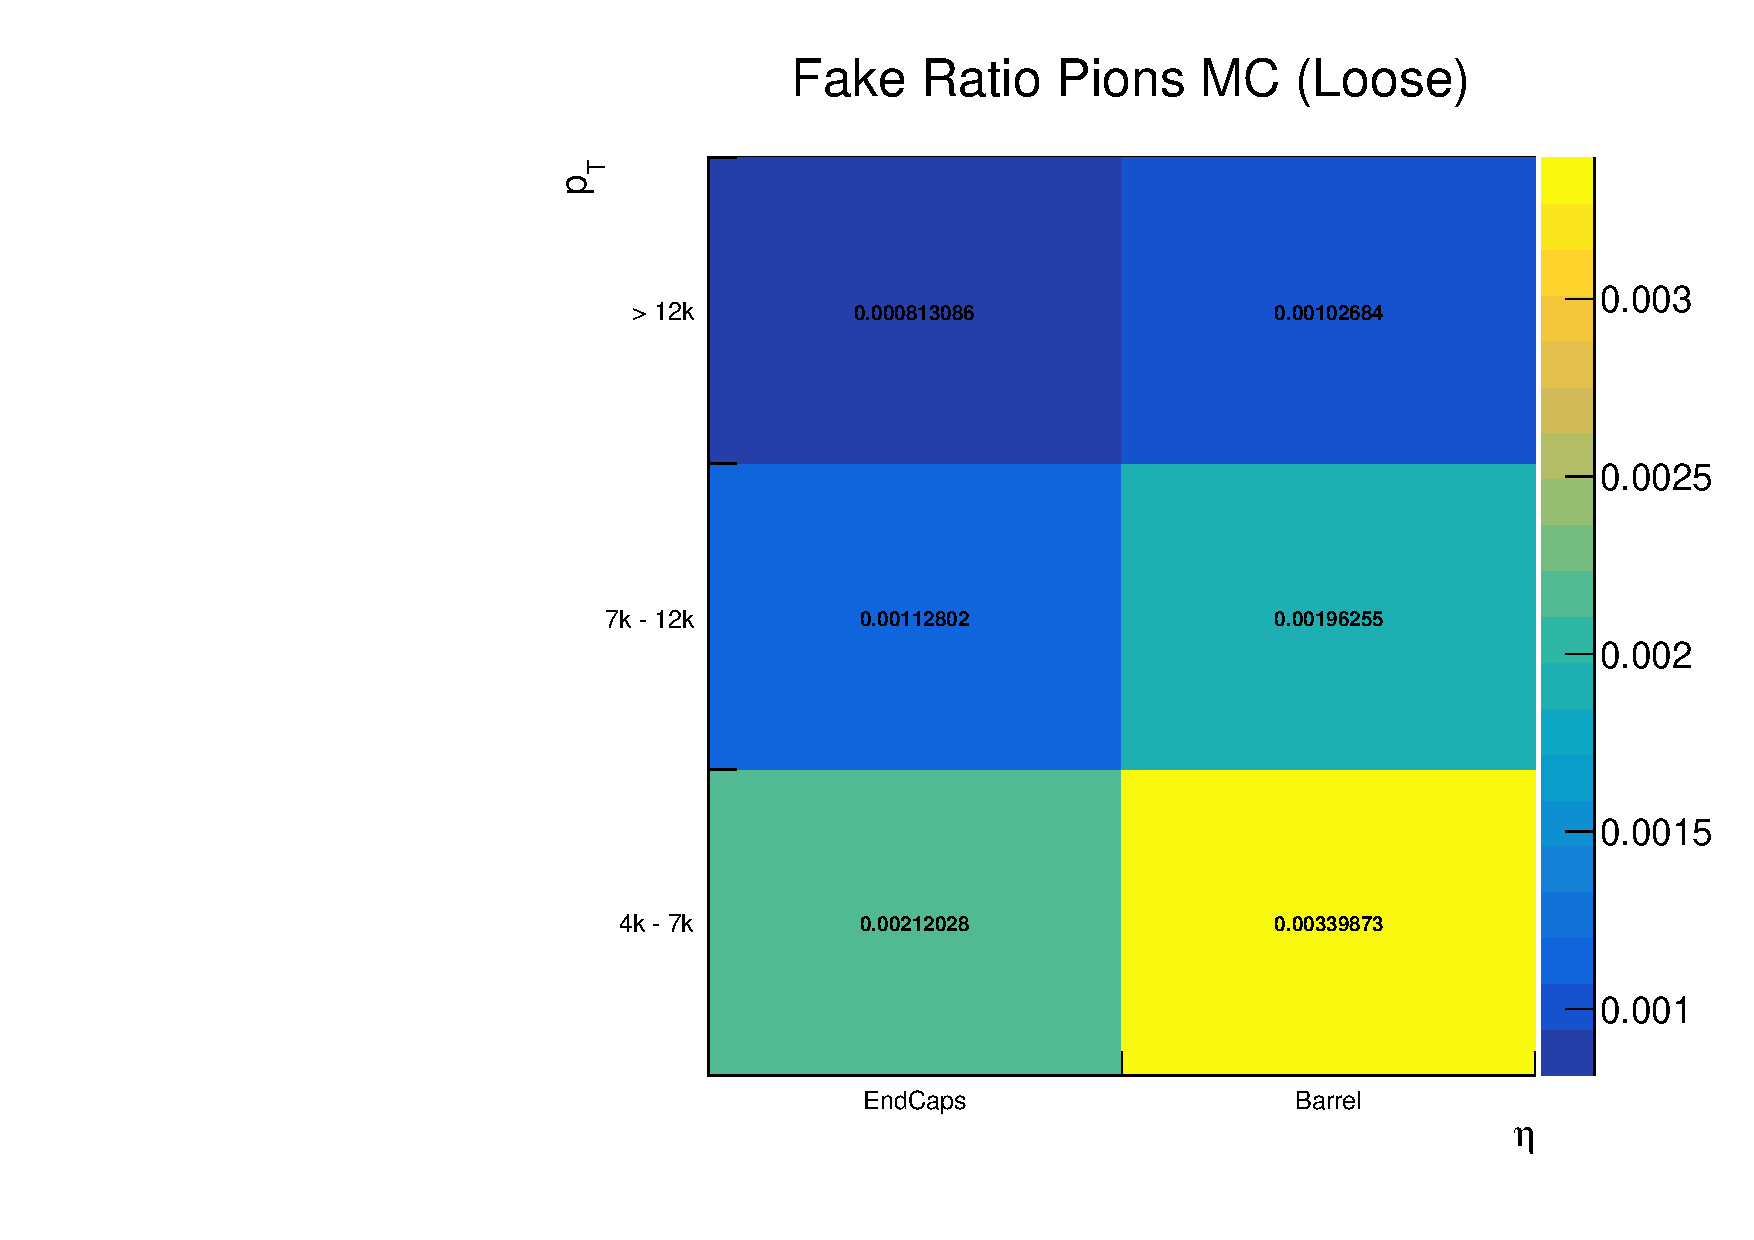
\includegraphics[width=0.45\textwidth]{figures/FakeRatesFit/FakeRatesPions/FakeRatesPionsLoose.pdf}
    \caption{ Fake Rates for $P(K^\pm \to \mu^\pm)$ (left) and $P(\pi^\pm \to \mu^\pm)$ (right) in Barrel and Endcap. Results for the tight working point are given in the Appendix-~\ref{subsec:Fake_Rates_Pion_TW}}
    \label{fig:K-to-ell-faking-probabilities}
\end{figure}
\subsubsection{Perform Analysis without Lepton Identification cuts}
We now want to perform the entire analysis on the MC samples of the decays identified in the previous step to check how they contribute to the signal region of the analysis. %
We carefully remove all analysis choices that either implicitly or explicitly impose lepton identification criteria. %
We then correct for this exclusion of lepton identification criteria by applying the faking probabilities derived in \ref{subsubsec:estimation-of-fake-background} to each of the events passing the rest of the analysis selection. %
There are two main ways in which the lepton identification criteria can be imposed:
\begin{itemize}
    \item Offline lepton identification criteria are imposed on the reconstructed lepton objects, e.g., requiring that the ratio between the energy deposited in the hadronic calorimeter and the energy deposited in the electromagnetic calorimeter is less than a certain threshold, etc. We simply remove these criteria from the analysis selection. %
    \item Online lepton identification criteria are imposed on the reconstructed lepton objects during the trigger selection. The specific criteria are in one-to-one correspondence with the offline lepton identification criteria, however, they are applied on the lepton objects reconstructed by the trigger software instead of the more carefully reconstructed lepton objects in the offline analysis. We thus do not impose any trigger selection criteria while performing the analysis on the MC samples of the final state signatures. %
\end{itemize}
Additionally, there is a hidden way in which the offline lepton identification criteria are intertwined with the usual analysis workflow, namely, through the lepton-specific kinematic reconstruction. The kinematics of the charged tracks that are identified as muons is reconstructed using the Combined (CB) muon approach wherein both the tracks in the ID and the matched track in the Muon Spectrometer (MS) are utilized to reconstruct the kinematics of the muons. However, the CB reconstruction is initiated only for those ID tracks that qualify as muons in some loose sense (namely, they can be matched to an MS track). Thus, if we do not want to impose the lepton identification criteria on the reconstructed lepton objects, then we also need to not ask for the CB tracks for these objects - otherwise, we will be implicitly imposing a lepton identification criterion. This forces us to use the kinematics of the ID tracks for the reconstructed lepton objects. We will correct for this difference in the kinematic reconstruction of the lepton objects later on. %


\subsubsection{Applying the Faking Probabilities}
\label{subsec:applying-the-faking-probabilities}
The probability that a reconstructed $B$-candidate (before lepton identification) will be reconstructed as a signal candidate (after lepton identification) is given by the product of the faking probabilities of the charged hadron tracks $h_i$. %
There can be two cases: only $1$ fake plus $1$ real lepton or $2$ fake leptons. %
%In both cases, the particles that are faking the leptons are reconstructed under the blind assumption that they are leptons.
\begin{align}
    w_{\text{fake}} &= \Pi_{i=1}^{N=1,2}P_{h_i \to \mu_i}
\end{align}
where $N$ is the number of fake electrons in the reconstructed $B$-candidate, as determined from the truth identity of the faking particle in the MC sample. %
The role of combinatorics concerning which of the (possibly many) hadrons in the final state take the role of (one or two of) the leptons is already taken into account during the reconstruction of the $B$-candidates. %
%\DM{Make sure the reconstruction of the $B$-candidate shows up with some explanation in a search!!!}
Thus, the combinatorics do not need to be accounted for in calculating the faking probabilities for the $B$-candidates. %
The relevant ingredient probabilities are read from the faking probabilities of hadrons that are derived in \ref{subsubsec:estimation-of-faking-probabilities}. Notice that the faking probabilities are parametrized in the $p_{\text{T}}$ and $\eta$ of the ID track of the charged hadron, thus, a more explicit notation for $P_{h_i \rightarrow \mu_i}$ would read $P_{h_i \rightarrow \mu_i}(p_{\text{T}}^{\text{ID}}(h_i), \eta^{\text{ID}}(h_i))$. % 
Another important point to note is that since the faking probabilities are dependent on the type of hadron that is faking the lepton, we must utilize the MC truth information to identify the type of the hadron $h_i$ in question ($K^\pm$ or $\pi^\pm$). %
%\DM{EXPLAIN COMBINATORICS. HARD TO EXPLAIN WITHOUT USING ATLAS JARGON.}
\subsubsection{Kinematic Corrections}
\label{subsec:kinematic-corrections}
When the analysis is performed without requiring lepton identification cuts, this implicitly involves using ID tracks instead of the CB tracks for muons. This induces differences in the reconstructed kinematics of the tracks, leading to differences in the reconstructed mass of the $B-$meson (the discriminating variable that is ultimately fit). Thus, it becomes crucial to correct for these differences.
The MC samples of the reference channel (\Bmumu ) are used to derive this correction. %
Notice that a `bin-by-bin correction' approach cannot be applied since a given value of CB $p_{\text{T}}$ corresponds to multiple values of ID $p_{\text{T}}$. %
Thus, bin-by-bin corrections derived using one sample will not be applicable to another sample. %
Rather, we adopt the following approach wherein the response of $p_{\text{T}}$ is evaluated as
    \begin{align}
        \mathcal{R}_{p^+_{\text{T}}} &= \frac{p^+_{\text{T}}({\text{CB}}) - p^+_{\text{T}}({\text{ID}})}{p^+_{\text{T}}({\text{ID}})}\\
    \end{align}
This response is parametrized in the $3{\text{D}}$ space of the $p_{\text{T}}$ of the two leptons and the angular distance between the two leptons, $\Delta R$- where all three variables are calculated using the {\text{ID}} tracks. Using these responses, following the process detailed in Appendix~\ref{sec:kinematic-corrections}, the kinematics of the fake MC samples are corrected. The kinematics correction result is presented in Figure \ref{fig:KinematicsCorrectionResults} (left). 

\begin{figure}[!ht]
    \centering 
    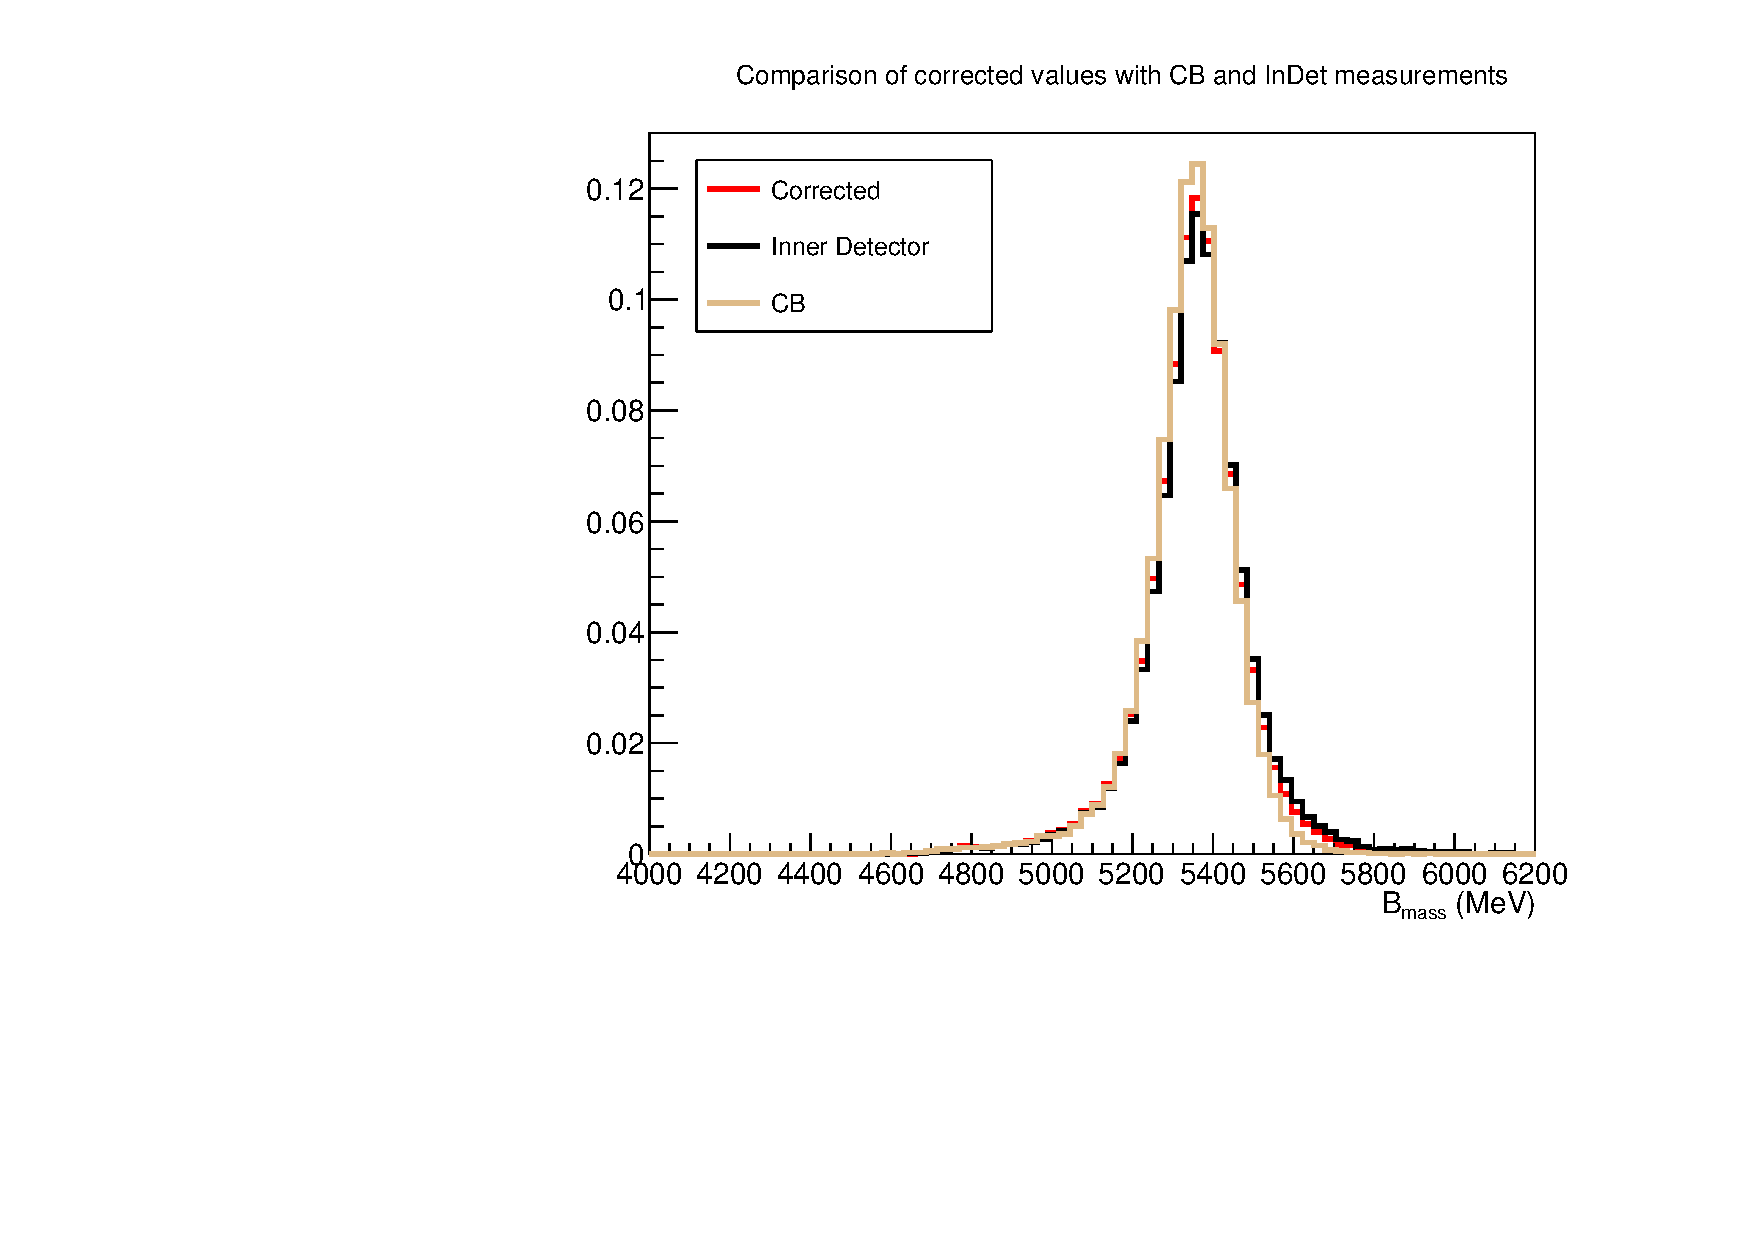
\includegraphics[width=0.43\textwidth]{figures/FakeRatesFit/KinematicsCorrectionResults.pdf}
    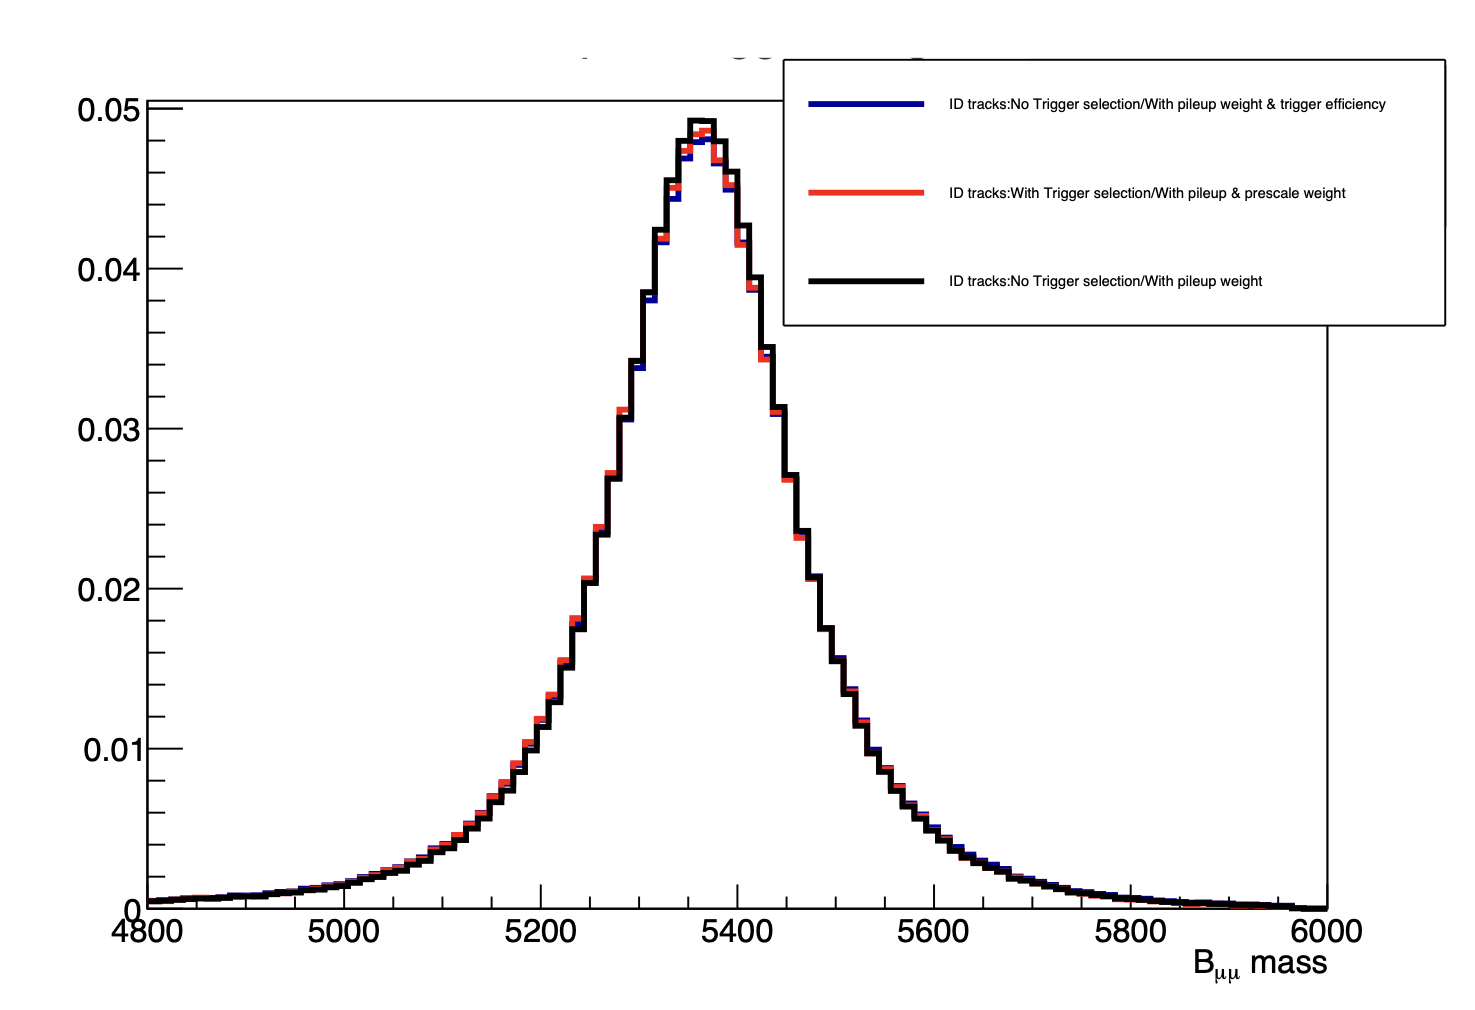
\includegraphics[width=0.47\textwidth]{figures/FakeRatesFit/TriggerWeights.png}
    \caption{Left: Comparison of the Combined muon $B_{\text{mass}}$ distribution with the Inner Detector measurement and the implementation of the kinematics correction on the Inner Detector values. Right: Comparison of the applied trigger corrections on Inner Detector tracks. }
    \label{fig:KinematicsCorrectionResults}
\end{figure}

\subsubsection{Applying Trigger Weights}
\label{subsec:applying-trigger-weights}
To correct for the lack of trigger-level lepton identification criteria, we derive the probability that a given $B$-candidate will pass the trigger selection, given that it has passed the offline selection. %
Recall that we have already corrected for the lack of offline lepton identification criteria by applying the faking probabilities to the $B$-candidates. %
Thus, we assume that if a hadron passes the offline lepton identification criteria, then its conditional probability of passing the trigger-level lepton identification criteria can be approximated by the same probability for a real lepton. %
Consequently, we can use the reference channel to derive the trigger weights. %
Currently, these weights are derived using the MC samples of the reference channels. %\DM{Say anything about data-driven?} %
These weights, intuitively, correspond to the probability that a given $B$-candidate will pass the trigger selection, given that it has passed the offline selection -- correspondingly, they are derived using the ratio of the number of events passing the trigger selection (and the offline lepton selection) to the number of events passing the offline selection. %
However, to take into account the effect of prescales that are not simulated in the MC samples, each of the events in the numerator of the ratio is weighted by the prescale weight. %The details of how the prescale weights are derived are discussed in \secref{sec:prw-for-beex}. %
The trigger weights are parametrized in the $p_{\text{T}}, \eta$ of the two leptons and the $\Delta R$ between the two leptons. %
In order to avoid having to optimize binning in this $5{\text{D}}$ space, the parametrization is achieved using Gaussian Kernel Density Estimation (KDE). %
Thus, the trigger weights are given by:
\begin{align}
    w_{\text{trigger}}( p_{\text{T}}^+, p_{\text{T}}^-, \eta^+, \eta^-, \Delta R) &= \frac{\rho_{\text{trigger + prescale + offline}}(p_{\text{T}}^+, p_{\text{T}}, \eta^+, \eta^-, \Delta R)}{\rho_{\text{offline}}(p_{\text{T}}^+, p_{\text{T}}^-, \eta^+, \eta^-, \Delta R)}
\end{align}
where $\rho_{\text{trigger + prescale + offline}}$ is the density of the events passing the trigger selection (and the offline lepton selection) weighted by the prescale weight, and $\rho_{\text{offline}}$ is the density of the events passing the offline selection. %
A comparison of the trigger weights effectiveness is given in Figure \ref{fig:KinematicsCorrectionResults} (right). 

